% Trevor Austin (u11310856)
The issues related to usability and the testing of usability are included below:
\subsubsection{Notification A Usability Testing}
\begin{itemize}
	\item The first and foremost problem is there is no way to test if the notification section is usable as no testing infrastructure for usability is provided. The team would need to implement just a basic interface to allow users to actually use the functions they have implemented. Thus, without this in place the notification module has no real usability. In order to provide a full usability testing section, the authors have assumed that there is a functioning interface for some of the points below.
	\item There was no testing interface that functioned correctly. This prevented further usability tests as the tester could not see if the functions were procedurally correct. All 18 of the 18 tests failed when attempting to use nodeunit(the testing infrastructure that was provided). This can be seen in the figure \ref{fig:usabFailA}. This shows further that the module, even with a functioning interface, would not be able to have any usability.
	/begin{figure}[h!]
		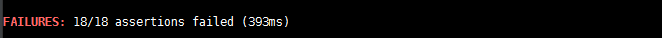
\includegraphics[width=\linewidth]{../images/Failure.png}
		\caption{Usability test failure}
		\label{fig:usabFailA}
	/end{figure}
	\item The call-back nature of many of the functions, as mentioned in previous sections, is lacking. Many of the functions that are called return Boolean values but they do not use call-back functions in order to return these functions. This in combination with the asynchronous nature of JavaScript, or node.js, causes the values to always return true values. With relation to usability, the user would always assume that when they register for a notification, unregister, or even opt in for e-mail notifications. This proves to be false as the functions do not return properly which can cause frustration for the user as the program does alter values as expected. The usability for the function calls within the module is null.
	\item Similar to the above point, none of the functions throw errors. This prevents notification to user of problems within the application. The user would become frustrated as they would not be able to understand why the program is not functioning correctly. The user would not be able to provide specific debugging information as feedback to the developers.
	\item NPM install of the module does not function at all(See Figure \ref{fig:npmFailA} below) . So with regards to usability for developers the module has failed.
	/begin{figure}[h!]
		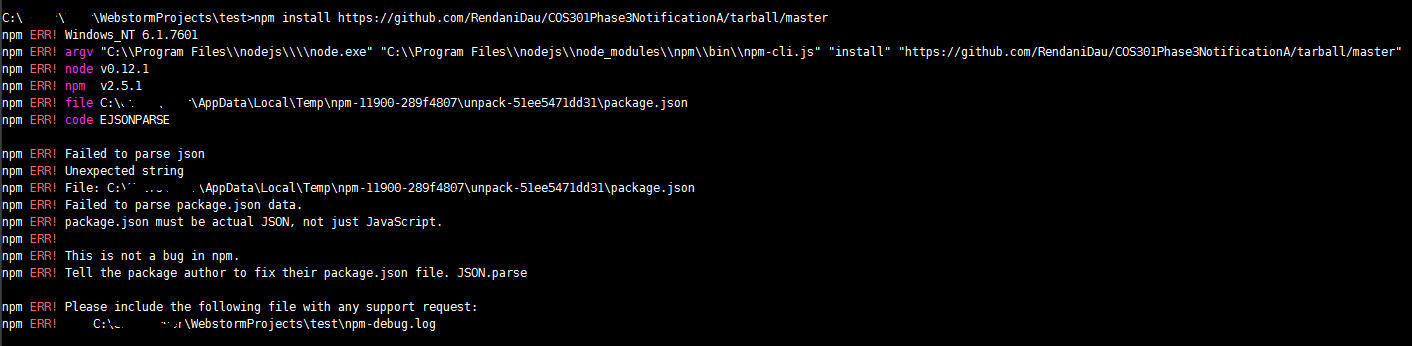
\includegraphics[width=\linewidth]{../images/npmfail.png}
		\caption{Usability test failure}
		\label{fig:npmFailA}
	/end{figure}
\end{itemize}
\subsubsection{Notification B Usability Testing}
\begin{itemize}
\item
\end
\subsubsection{Remarks}

